\newif\ifvimbug
\vimbugfalse

\ifvimbug
\begin{document}
\fi

\exercise{Trajectory Generation with Dynamical Systems}
In this exercise we will use the Dynamic Motor Primitives (DMPs), described by the following dynamical system,
%
\begin{align}
    \ddot{y}&=\tau^2(\alpha(\beta(g-y)-(\dot{y}/\tau))+f_w(z)), \label{eq:dmp} \\
    \dot{z}&=-\tau\alpha_zz, \label{eq:dmp_phase}
\end{align}
%
where $y$ is the state of the system, $\dot{y}$ and $\ddot{y}$ are the first and second time derivatives, respectively. The attractor's goal is denoted by $g$ and the forcing function by $f_w$. The parameters $\alpha$ and $\beta$ control the spring-damper system. The phase variable is denoted by $z$ and the temporal scaling coefficient by $\tau$. The forcing function $f_w$ is given by
%
\begin{equation}
    f_w(z)=\frac{\sum_{i=0}^{K}\phi_{i}(z)w_{i}z}{\sum_{j=0}^{K}\phi_{j}(z)}=\vec{\psi}(z)^{T}\vec{w},
    \quad \textrm{with}\quad \psi_i(z) = \frac{\phi_i(z)z}{\sum_{j=1}^K\phi_j(z)},
\end{equation}
%
where the basis functions $\phi_i(z)$ are Gaussian basis given by
%
\begin{equation}
    \phi_i(z) = \exp(-0.5(z-c_i)^2/h_i),
\end{equation}
where the centers $c$ are equally distributed in the phase $z$, and the width $h$ is an open parameter. For the programming exercises a basic environment of a double link pendulum is provided, as well as the computation of the $\vec{\psi}_i(z)$.


\begin{questions}

%----------------------------------------------

\begin{question}{Similarities to a PD controller}{2}
Transform Equation~\eqref{eq:dmp} to have a similar structure to a PD-controller,
%
\begin{equation}
    \ddot{y}_z = K_P ( y^{des}_z - y_z ) + K_D ( \dot{y}_z^{des} - \dot{y}_z ) +
    u_{ff}
\end{equation}
%
and write down how the following quantities $K_p, K_d, y^{des}_z$ and $\dot{y}_z^{des}$ look like in terms of the DMP parameters. Do not expand the forcing function $f_w(z)$ at your solutions.

\begin{answer}
\begin{align*}
	\ddot{y}_{z} & = \tau^2\alpha\beta\cdot (g-y) + \alpha\cdot\tau\cdot(0-\dot{y}) + \tau^2 f_{w}(z)\\
	K_p & = \tau^2\alpha\beta\\
	K_d & = \alpha \cdot \tau\\
	y_{z}^{des} & = g\\
	\dot{y}_{z}^{des} & = 0\\
\end{align*}
\end{answer}

\end{question}

%----------------------------------------------

\begin{question}{Stability}{2}
Show why the DMPs are stable when $t\to\infty$ and what would the equilibrium point be.

\begin{answer}
	A high t means our forcing function goes to zero. This leaves us with a PD-controller that only controls $\ddot{y}_{z}$ to compensate for gravity. The equilibrium point would be at $y_{z}^{des}$ which is $g$.
\end{answer}

\end{question}

%----------------------------------------------

\begin{question}{Double Pendulum - Training}{12}
Implement the DMPs and test them on the double pendulum environment.
In order to train the DMPs you have to solve Equation~\eqref{eq:dmp} on the forcing function. Before starting the execution, set the goal $g$ position to be the same as in the demonstration. Then, set the parameters to $\alpha=25, \beta=6.25, \alpha_z=3/T, \tau=1$. Use $N=50$ basis functions, equally distributed in $z$.  Use the learned DMPs to control the robot and plot in the same figure both the demonstrated trajectory and the reproduction from the DMPs.
You need to implement the DMP-based controller (\texttt{dmpCtl.py}) and the training function for the controller parameters (\texttt{dmpTrain.py}). To plot your results you can use \texttt{dmpComparison.py}. Refer to \texttt{example.py} to see how to call it. Attach a snippet of your code.

\begin{answer}
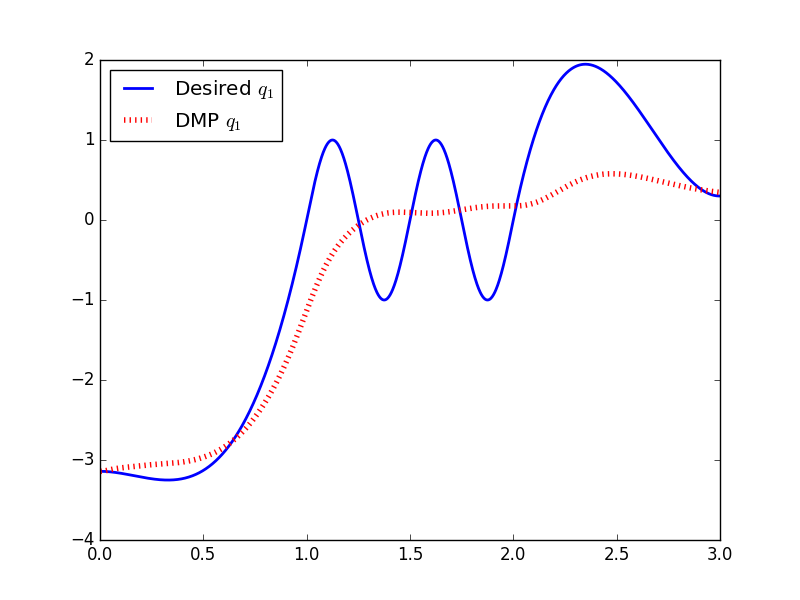
\includegraphics[width=87mm]{python/figures/figure_1.png}
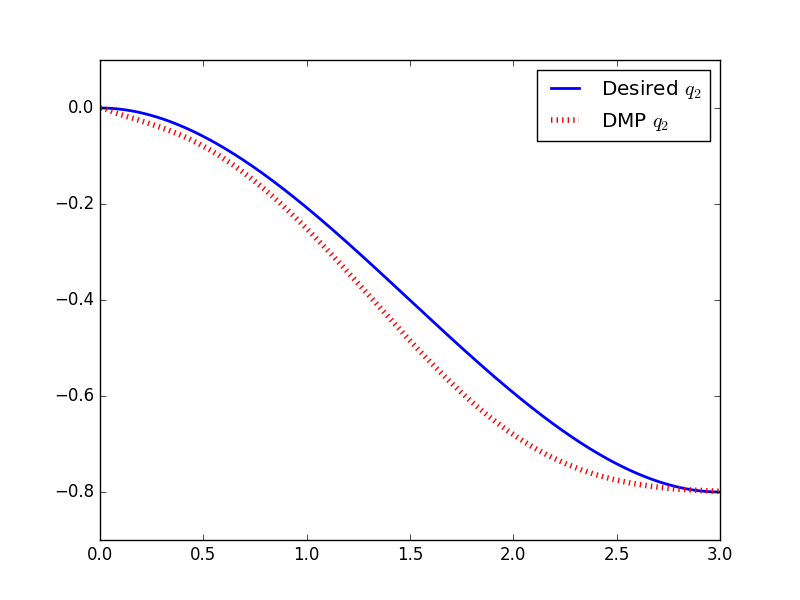
\includegraphics[width=87mm]{python/figures/figure_2.png}
\texttt{the control code:}\\
\lstinputlisting[language=Python, firstline=11,lastline=21]{python/dmpCtl.py}
\texttt{the training code:}\\
\lstinputlisting[language=Python, firstline=27,lastline=65]{python/dmpTrain.py}
\end{answer}

\end{question}



%----------------------------------------------

\begin{question}{Double Pendulum - Conditioning on the Final Position}{3}
Using the trained DMPs from the previous question, simulate the system with different goal positions: first with $q_{t=\mathrm{end}} = \{0, 0.2\}$ and then with $q_{t=\mathrm{end}} = \{0.8, 0.5\}$. Generate one figure per DoF. In each figure, plot the demonstrated trajectory and the reproduced trajectories with different goal positions.
How do you interpret the result? 

\begin{answer}
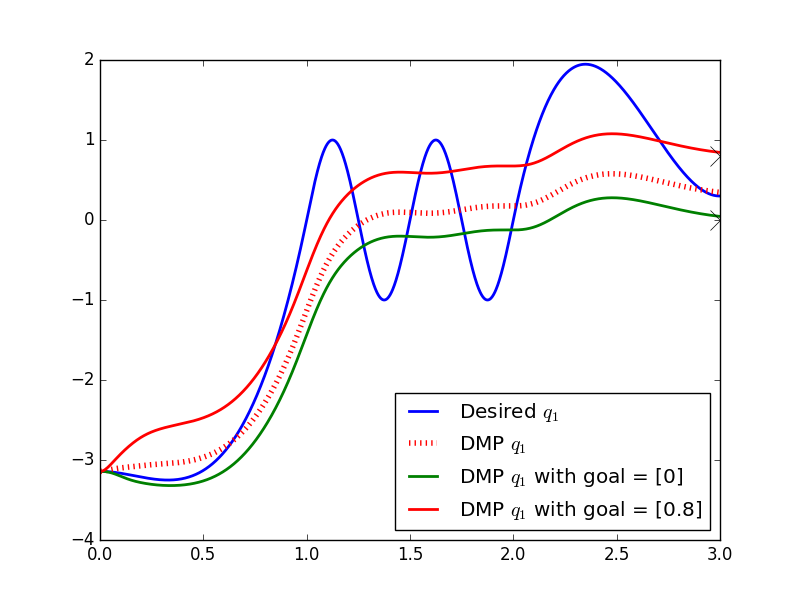
\includegraphics[width=87mm]{python/figures/figure_3.png}
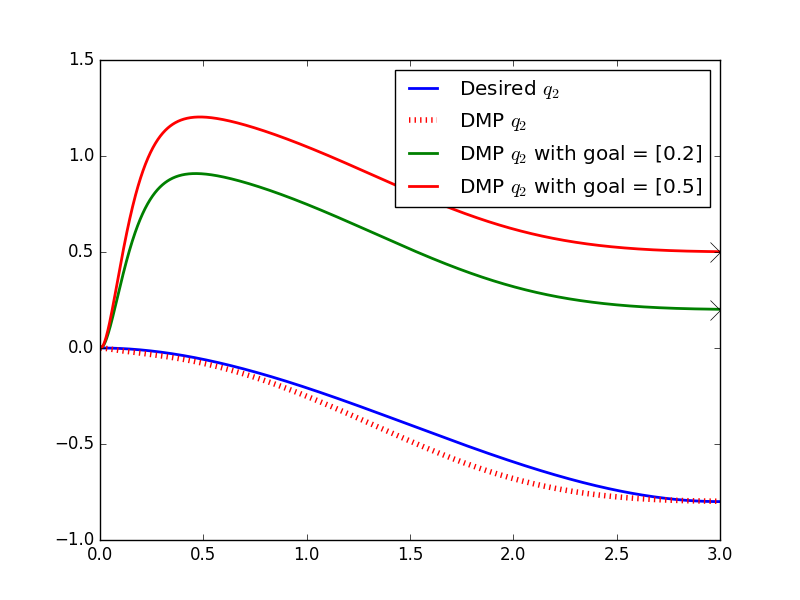
\includegraphics[width=87mm]{python/figures/figure_4.png}
\end{answer}


\end{question}

%----------------------------------------------

\begin{question}{Double Pendulum - Temporal Modulation}{3}
Using the trained DMPs from the previous question, simulate the system with different temporal scaling factors $\tau=\{0.5, 1.5\}$. Generate one figure per DoF and explain the result.

\begin{answer}
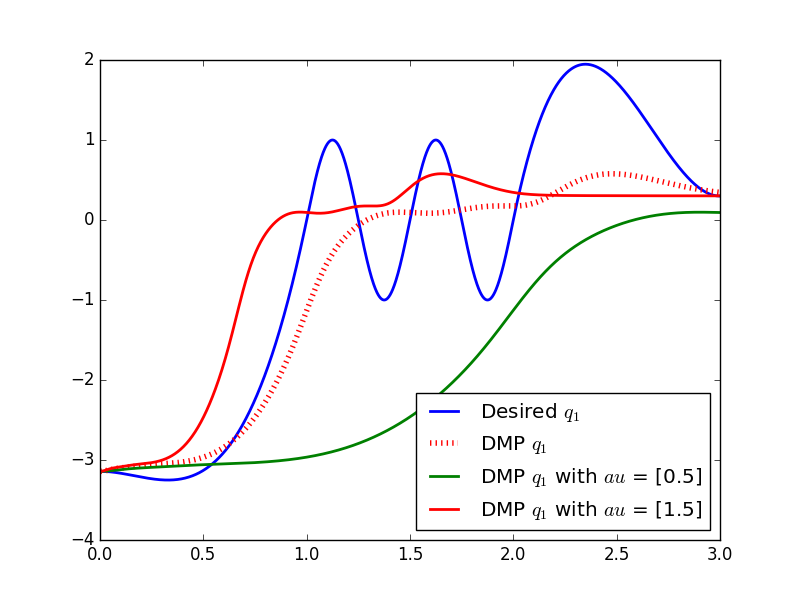
\includegraphics[width=87mm]{python/figures/figure_5.png}
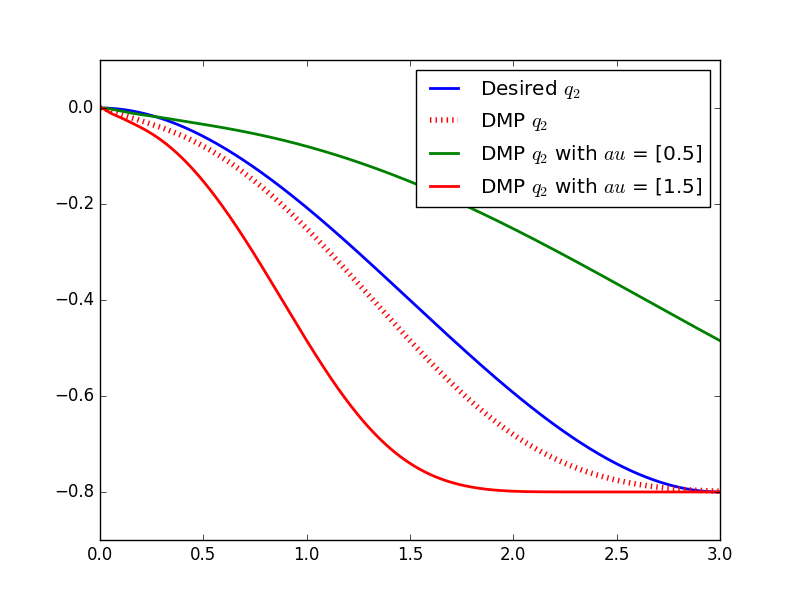
\includegraphics[width=87mm]{python/figures/figure_6.png}
\end{answer}


\end{question}

%----------------------------------------------

\begin{question}[bonus]{Probabilistic Movement Primitives - Radial Basis Function}{3}
We now want to use ProMPs. Before we train them, we need to define some basis functions. We decide to use $N = 30$ radial basis functions (RBFs) with centers uniformly distributed in the time interval $[0-2b,T+2b]$, where $T$ is the end time of the demonstrations.
The bandwidth of the Gaussian basis (std) is set to $b=0.2$. 
Implement these basis functions in \texttt{getProMPBasis.py}. 
Do not forget to normalize the basis such at every time-point they sum-up to one! Attach a plot showing the basis functions in time and a snippet of your code. 

\begin{answer}
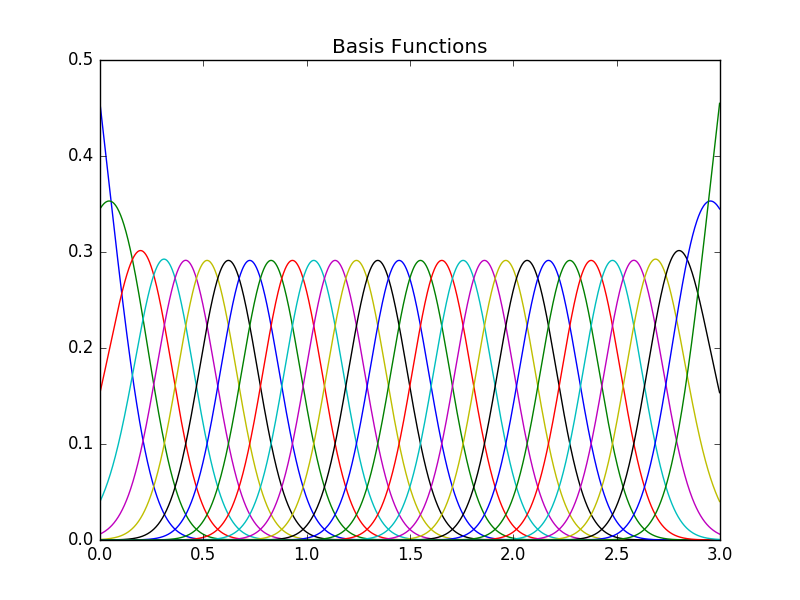
\includegraphics[width=170mm]{python/figures/figure_7-basisfunctions.png}
\lstinputlisting[language=Python, firstline=4,lastline=22]{python/getProMPBasis.py}
\end{answer}
\end{question}

%----------------------------------------------

\begin{question}[bonus]{Probabilistic Movement Primitives - Training}{7}
In this exercise you will train the ProMPs using the imitation learning data from \texttt{getImitationData.py} and the RBFs defined in the previous question. Modify the \texttt{proMP.py} in order to estimate weight vectors $w_i$ reproducing the different demonstrations. Then, fit a Gaussian using all the weight vectors. Generate a plot showing the desired trajectory distribution in time (mean and std) as well as the trajectories used for imitation. Attach a snippet of your code.

\begin{answer}
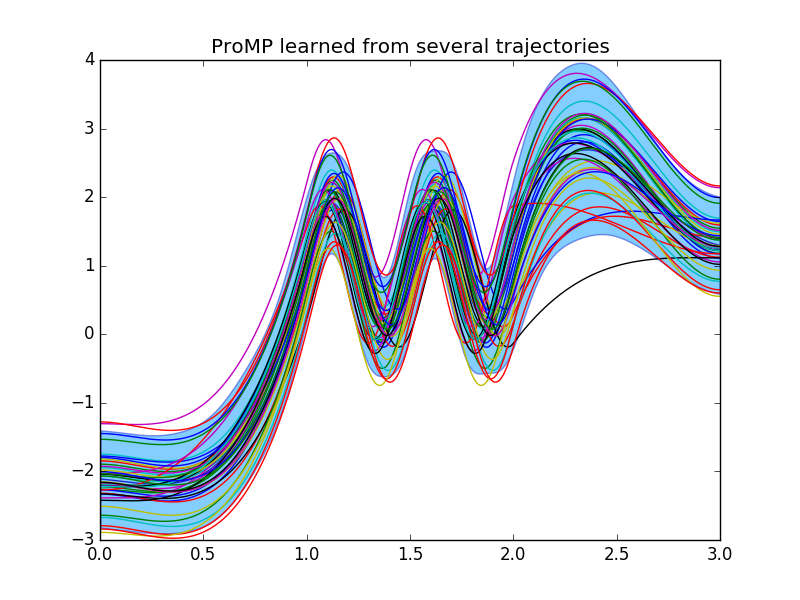
\includegraphics[width=170mm]{python/figures/figure_8-trajectories.png}
\lstinputlisting[language=Python, firstline=6,lastline=27]{python/proMP.py}
\end{answer}

\end{question}

%----------------------------------------------

\begin{question}[bonus]{Probabilistic Movement Primitives - Number of Basis Functions}{2}
Evaluate the effects of using a reduced number of RBFs. Generate two plots showing the desired trajectory distribution and the trajectories used for imitation as in the previous exercise, but this time use $N=20$ and $N=10$ basis functions. Briefly analyze your results.

\begin{answer}
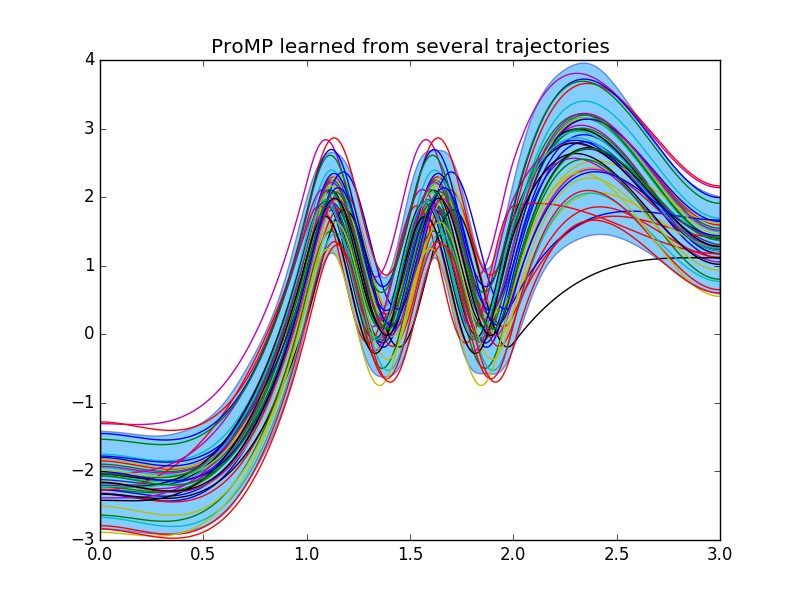
\includegraphics[width=87mm]{python/figures/figure_9-trajectoriesN20.png}
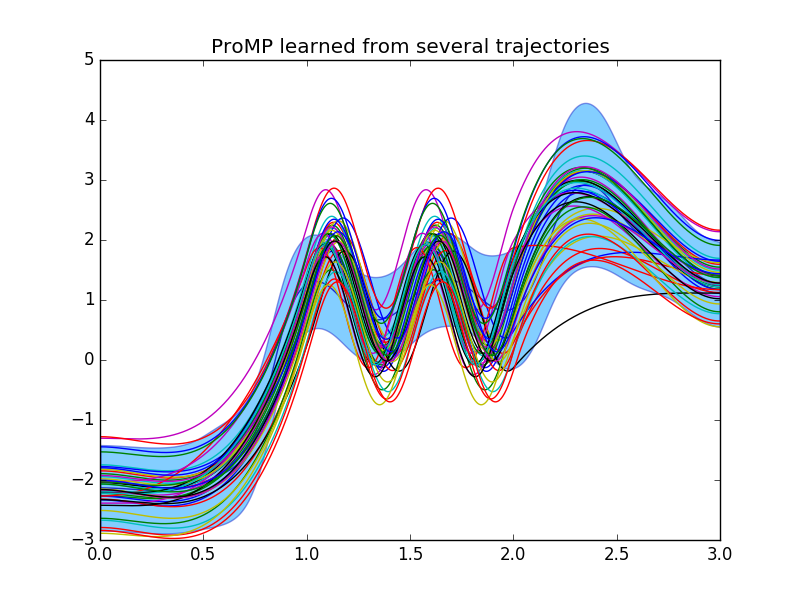
\includegraphics[width=87mm]{python/figures/figure_10-trajectoriesN10.png}
\\
On the left side were 10 radial basis functions used. On the right side 20. 
One can easily see, that the reduction to N=20 basis functions does'nt affect the result too much, but the reductionn to N=10 does. The trajectory distribution doesn't fit the trajectories equally well anymore as with 20 functions.
\end{answer}

\end{question}

%----------------------------------------------


\begin{question}[bonus]{Probabilistic Movement Primitives - Conditioning}{4}
Using Gaussian conditioning calculate the new distribution over the weight vectors $w_i$ such as the trajectory has a via point at position $y^*=3$ at time $t_\textrm{cond}=1150$ with variance $\Sigma_{y^*}=0.0002$.
Assuming that the probability over the weights is given by $\mathcal{N}(\vec w|\vec \mu_w,\vec \Sigma_w)$ and the probability of being to that position is given by $\mathcal{N}(y^*|\vec \Phi \vec w, \Sigma_{y^*} )$, show how the new distribution over $\vec w$ is computed (how does the mean and variance look like)?
\\
Then, in a single plot, show the previous distribution (learned from imitation) and the new distribution (after conditioning). Additionally, sample $K=10$ random weight vectors from the ProMP, compute the trajectories and plot them in the same plot. Analyze briefly your results and attach a snippet of your code.

\begin{answer}
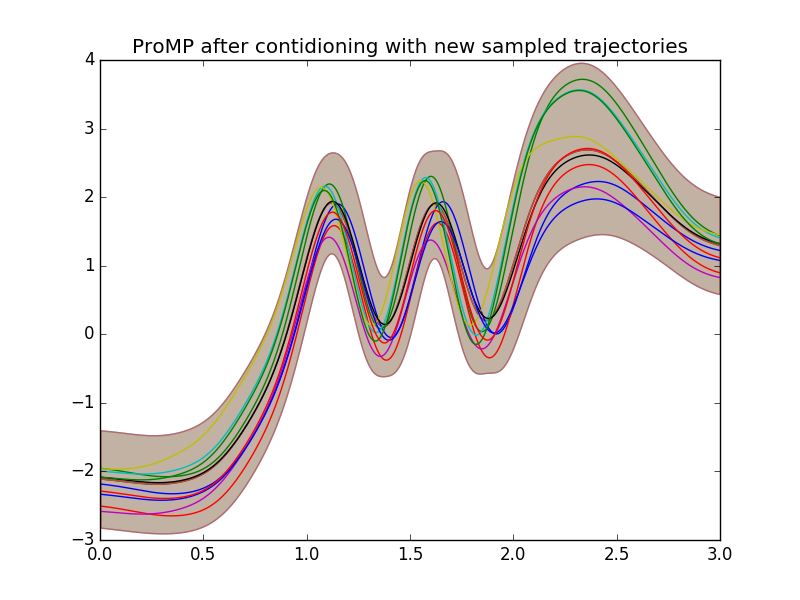
\includegraphics[width=170mm]{python/figures/figure_13-conditioningN10.png}
\lstinputlisting[language=Python, firstline=28]{python/proMP.py}
\end{answer}

\end{question}

\end{questions}
